\begin{center}
    {\bf МАГНИТНЫЙ ГЕОДЕЗИЧЕСКИЙ ПОТОК НА МНОГООБРАЗИИ ВРАЩЕНИЯ: ТОПОЛОГИЧЕСКИЕ ИНВАРИАНТЫ}

    {\it И.Ф. Кобцев}

    (Москва; {\it int396.kobtsev@mail.ru})
\end{center}

Рассмотрим многообразие $M \approx S^2$, на котором определено действие группы $S^1$ изометриями (такое многообразие называется многообразием вращения). Оно имеет метрику $ds^2=dr^2+f^2(r)d\varphi^2$. Определим на $T^*M$ магнитный геодезический поток как гамильтонову систему с гамильтонианом $H = \frac{p_r^2}{2}+\frac{p_\varphi^2}{2f^2(r)}$ и симплектической структурой $\widetilde{\omega}=dp_r \wedge dr + dp_\varphi \wedge d\varphi+\Lambda'(r)dr \wedge d\varphi$.

В [1] использовался другой подход к получению новых систем на многообразии вращения "--- добавление потенциала: $H = \frac{p_r^2}{2}+\frac{p_\varphi^2}{2f^2(r)}+V(r)$. Рассмотрение магнитного поля вместо потенциала приводит к ряду новых топологических свойств.

Предположим, что выполнены следующие условия на функции $f(r)$ и $\Lambda(r)$ [1]:
\begin{enumerate}
	\item $f(r):(0,L)\to \mathbb{R}$ продолжается до гладкой нечётной $2L$-периодической функции Морса $f(r):\mathbb{R}\to \mathbb{R}$, $f'(0)=1$, $f'(L)=-1$;
	\item $\Lambda(r):(0,L)\to \mathbb{R}$ продолжается до гладкой чётной $2L$-периодической функции Морса $\Lambda(r):\mathbb{R}\to \mathbb{R}$;
	\item $(\Lambda'(r))^2+(f'(r))^2>0$,
\end{enumerate}
где $L$ "--- длина геодезической, соединяющей полюса. Этот набор условий обеспечивает гладкость $H$ и $\widetilde{\omega}$ на $T^*M$.

Целью исследования является вычисление инвариантов Фоменко-Цишанга, характеризующих топологию слоения Лиувилля на неособом изоэнергетическом многообразии $Q_h=\{H=h\}$.

\textbf{Утверждение~1.} {\it Определённая таким образом система имеет две степени свободы и является вполне интегрируемой по Лиувиллю; дополнительным интегралом является $K=p_\varphi-\Lambda(r)$.}

Фазовое пространство этой системы расслаивается на инвариантные (относительно фазового потока системы) двумерные слои, являющиеся совместными поверхностями уровня интегралов $H=h$, $K=k$, т.е. корректно определено слоение, называемое слоением Лиувилля. Согласно теореме Лиувилля это слоение состоит из слоёв двух типов:
\begin{itemize}
	\item регулярные слои, диффеоморфные несвязному объединению торов $T^2$ (называемых торами Лиувилля);
	\item особые слои (бифуркации торов Лиувилля).
\end{itemize}

Структура слоения Лиувилля интегрируемых гамильтоновых систем с двумя степенями свободы известна и описана в [2].

В ходе исследования получены следующие результаты:
\begin{itemize}
	\item построены бифуркационные диаграммы, найдены уравнения бифуркационных кривых;
	\item исследован топологический тип перестроек торов Лиувилля на неособом изоэнергетическом многообразии. В частности, обнаружены перестройки типов $A$, $V_s$ (встречавшиеся в [1]) и найдены новые бифуркации (рис. 1), у которых критические окружности ориентированы несогласованно [2, раздел 3.3];
	\item по виду бифуркационных диаграмм вычислены инварианты Фоменко и Фоменко--Цишанга;
	\item обнаружено совпадение ряда инвариантов с уже встречавшимися в других задачах механики. Это позволяет сделать вывод о лиувиллевой эквивалентности систем с совпадающими инвариантами.
\end{itemize}
\begin{figure}
\begin{minipage}{0.33\linewidth}
\begin{center}
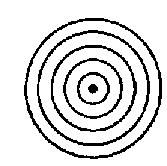
\includegraphics[scale=0.3]{atomA.jpg} \\ a)
\end{center}
\end{minipage}
\hfill
\begin{minipage}{0.33\linewidth}
\begin{center}
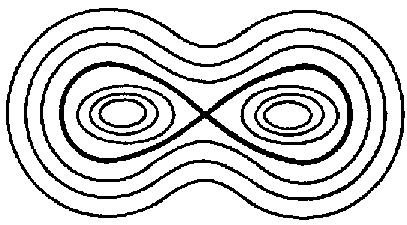
\includegraphics[scale=0.2]{atomB.jpg} \\ б)
\end{center}
\end{minipage}
\hfill
\begin{minipage}{0.98\linewidth}
\begin{center}
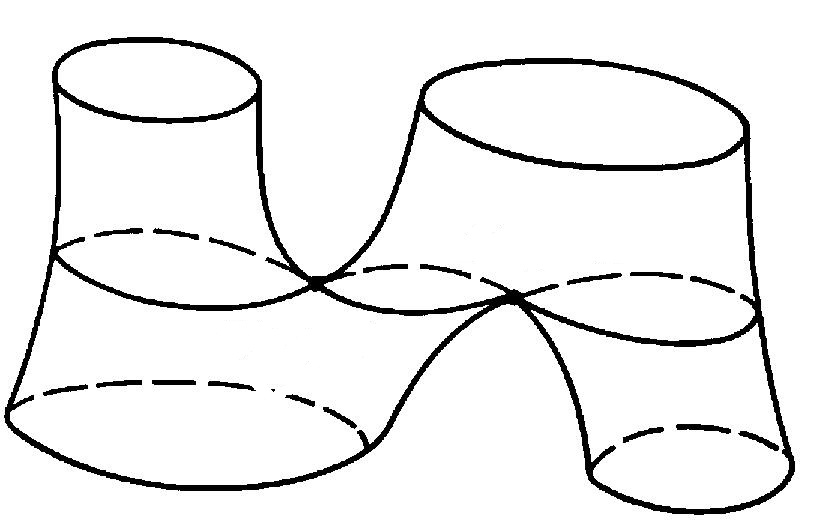
\includegraphics[scale=0.2]{unstable.jpg} \\ в)
\end{center}
\end{minipage}
\caption{\small{Двумерные базы 3-мерных окрестностей особых слоёв слоения Лиувилля на неособом изоэнергетическом многообразии: а "--- типа $A$; б "--- типа $V_2=B$; в "--- пример 4-мерной перестройки торов Лиувилля с несогласованными ориентациями критических окружностей (показана зависимость двумерной базы от уровня энергии h). Трёхмерная (соотв. четырёхмерная) бифуркация получается в результате умножения двумерной базы (при каждом значении h) на окружность.}}
\end{figure}

% Оформление списка литературы
\smallskip \centerline {\bf Литература} \nopagebreak

1. {\it Кантонистова Е. О.} Топологическая классификация интегрируемых гамильтоновых систем на поверхностях вращения в потенциальном поле.
Матем.сб.,2016, том 207, №3, с. 47--92.

2. {\it Болсинов А. В., Фоменко А. Т.} Интегрируемые гамильтоновы системы. Геометрия, топология, классификация. Ижевск: Издательский дом <<Удмуртский университет>>, 1999.
